\documentclass[12pt,a4paper]{report}

\usepackage[T1]{fontenc}
\usepackage[utf8]{inputenc}
\usepackage{lmodern}
\usepackage[british]{babel}
\usepackage[margin=2.5cm]{geometry}
\usepackage{microtype}
\usepackage{amsmath}
\usepackage{booktabs}
\usepackage{tabularx}
\usepackage{array}
\usepackage{enumitem}
\usepackage{xcolor}
\usepackage{listings}
\usepackage{tikz}
\usetikzlibrary{arrows.meta,positioning,calc}
\usepackage[hidelinks]{hyperref}

\setlength{\parindent}{0pt}
\setlength{\parskip}{0.6em}

% "Section 3.2 [p. 7]" style cross-references.
\newcommand{\sref}[1]{Section~\ref{#1} [p.~\pageref{#1}]}
\newcommand{\cref}[1]{Chapter~\ref{#1} [p.~\pageref{#1}]}
\newcommand{\fref}[1]{Figure~\ref{#1} [p.~\pageref{#1}]}
\newcommand{\lref}[1]{Listing~\ref{#1} [p.~\pageref{#1}]}
\newcommand{\tref}[1]{Table~\ref{#1} [p.~\pageref{#1}]}
\newcommand{\eref}[1]{(\ref{#1}) [p.~\pageref{#1}]}
\DeclareRobustCommand{\code}[1]{\texttt{\detokenize{#1}}}
\newcommand{\commit}[1]{\texttt{#1}}

\definecolor{codebg}{RGB}{247,247,247}
\definecolor{codekw}{RGB}{0,70,140}
\definecolor{codecm}{RGB}{110,110,110}
\definecolor{codest}{RGB}{150,60,0}

\lstdefinestyle{py}{
  language=Python,
  basicstyle=\ttfamily\footnotesize,
  keywordstyle=\color{codekw}\bfseries,
  commentstyle=\color{codecm}\itshape,
  stringstyle=\color{codest},
  backgroundcolor=\color{codebg},
  numbers=left,
  numberstyle=\tiny\color{codecm},
  frame=single,
  rulecolor=\color{codecm},
  breaklines=true,
  showstringspaces=false,
  columns=fullflexible,
  keepspaces=true,
  upquote=true,
}
\lstset{style=py}
\renewcommand{\lstlistingname}{Listing}

% Source files are read straight from the repository, so line numbers in the
% listings are the real line numbers at the time of writing.
\newcommand{\src}[1]{../src/#1}

\begin{document}

\begin{titlepage}
  \centering
  \vspace*{2cm}
  {\large VEX V5 Competition Robot\par}
  \vspace{1.5cm}
  {\LARGE\bfseries Engineering Report:\\[0.3em] The Program\par}
  \vspace{1.5cm}
  {\large How the program is structured, what each part does, and how it\\
  developed between September and October 2026\par}
  \vfill
  {\large Utsav Choudhury\par}
  \vspace{0.5em}
  {October 2026\par}
\end{titlepage}

\pagenumbering{roman}
\tableofcontents
\clearpage
\pagenumbering{arabic}

\chapter{Introduction}
\label{ch:intro}

This report documents the program that runs our VEX V5 competition robot. The
robot has two drive wheels, an arm, a claw, and an AI Vision sensor (a camera
that can recognise colours). The program is written in Python using the VEXcode
extension for VS Code, and it runs on the V5 Brain, the small computer on the
robot that controls the motors and reads the sensors.

A competition match has two parts. In the \emph{autonomous} period, the robot
moves on its own using only its program, so every movement must be planned and
measured in advance. In the \emph{driver control} period, a driver steers the
robot with a handheld controller, so the program's job is to turn stick
movements into smooth, predictable motor power. The program therefore has two
main halves, and most of this report explains how each half works and why it
was built that way.

The report has three aims:

\begin{enumerate}
  \item To explain the \textbf{structure} of the program: which file holds what,
    and how the files are combined before they reach the robot.
  \item To explain \textbf{what each part does}, with references to the actual
    code and worked examples of the maths behind it.
  \item To record the \textbf{timeline} of development, the \textbf{challenges}
    we faced, and how we attempted to overcome them, including the attempts
    that did not work.
\end{enumerate}

The third aim matters because the final program is only a small part of the
story. For example, the autonomous routine went through more than forty
versions in two days before we replaced it with a simpler approach. Explaining
why we made that change is as useful as explaining the final code.

\section{Sources}

Everything in this report comes from the project's own records. These are the
source code in \code{src/}, the project documentation (\code{README.md} and
\code{AGENTS.md}), and the git history. Git is a version control system: every
time we saved a meaningful change, git recorded what changed, when, and a short
message explaining why. Each saved change is called a \emph{commit} and is
identified by a short code such as \commit{eb032a0}. We quote these codes
throughout so that every claim can be checked against the history. There are
57 commits between 22 September and 26 October 2026.

Code listings in this report are read directly from the source files, so their
line numbers match the real files at the time of writing. Code that has since
been removed is reproduced from the git history and labelled as such.

\section{Outline}

\cref{ch:structure} describes the hardware and how the code is organised.
\cref{ch:movement} explains autonomous movement, including the maths that turns
a distance into a motor rotation. \cref{ch:driver} explains driver control.
\cref{ch:vision} explains how the robot recognises the cone with the AI Vision
sensor. \cref{ch:timeline} gives the day-by-day timeline, and
\cref{ch:challenges} goes through the main challenges in detail.
\cref{ch:evaluation} evaluates the program's strengths and limitations, and
\cref{ch:conclusion} concludes the report.

\chapter{Program Structure}
\label{ch:structure}

This chapter describes the robot's hardware, how the code is split into files,
and the build step that combines those files before they are sent to the robot.
Understanding this structure first makes the later chapters easier to follow,
because each later chapter focuses on one of these files.

\section{Hardware}
\label{sec:hardware}

The V5 Brain has 21 numbered \emph{smart ports}. Each motor or sensor plugs into
one port, and the program must be told which port each device is on.
\tref{tab:ports} lists the devices.

\begin{table}[h]
  \centering
  \begin{tabular}{@{}cll@{}}
    \toprule
    Port & Device & Cartridge \\
    \midrule
    1  & Right drive motor & green, 18:1 \\
    2  & Left drive motor  & green, 18:1 \\
    4  & AI Vision sensor  & -- \\
    10 & Arm motor         & red, 36:1 \\
    15 & Claw motor        & red, 36:1 \\
    9  & VEXnet radio      & -- \\
    \bottomrule
  \end{tabular}
  \caption{Devices and the ports they are plugged into.}
  \label{tab:ports}
\end{table}

A \emph{cartridge} is the gearbox inside a V5 motor. A green 18:1 cartridge
gives a top speed of 200 revolutions per minute (rpm), which suits driving. A
red 36:1 cartridge gives 100 rpm but twice the torque (turning force), which
suits an arm that has to lift weight. The program must declare the correct
cartridge for each motor, because the motor uses it to convert its internal
rotation into output degrees. We return to what happens when this is wrong in
\sref{sec:gotchas}.

The radio on port 9 is managed by the Brain's own firmware, so the program
never declares it.

Note: in the Python SDK, ports are numbered from zero, so \code{Ports.PORT1} has
the value 0. This is why the port scanner in \sref{sec:portscan} adds 1 before
displaying a port number.

\section{File Layout}
\label{sec:layout}

The program is split into five Python files inside \code{src/}, plus one build
script. \tref{tab:files} summarises them.

\begin{table}[h]
  \centering
  \begin{tabularx}{\textwidth}{@{}lX@{}}
    \toprule
    File & Contents \\
    \midrule
    \code{config.py} & Every device and every tunable number. \\
    \code{vision.py} & Cone recognition and AI Vision diagnostics. \\
    \code{autonomousroutine.py} & Movement maths, calibration tools, and \code{autonomous()}. \\
    \code{drivercontrol.py} & Stick processing, the arm and claw, cone assist, and \code{user_control()}. \\
    \code{main.py} & Chooses which mode runs. \\
    \code{build.py} & Combines the five files into \code{src/download.py}. \\
    \bottomrule
  \end{tabularx}
  \caption{The files in the project and what each one holds.}
  \label{tab:files}
\end{table}

We keep every tunable number in \code{config.py}. This is useful because tuning
the robot usually means changing a speed, a distance, or a tolerance, and
having them in one place means we never have to search through the logic to
find them. Each constant has a short comment giving its unit or meaning, for
example:

\lstinputlisting[firstline=35,firstnumber=35,lastline=45,caption={Autonomous constants in \code{src/config.py}, lines 35--45.},label=lst:autoconst]{\src{config.py}}

\section{The Single-File Constraint}
\label{sec:singlefile}

The V5 Brain can only run \textbf{one} Python file. The project's settings are
stored in \code{vex_project_settings.json}, inside the \code{.vscode} folder.
This file has a single \code{main} entry that names the file to download, and
there is no way to list several files. This
creates a problem: a line such as \code{from config import *} works in the
editor, because the editor can see \code{config.py}, but fails on the robot with
an \code{ImportError}, because \code{config.py} was never sent.

Before 22 September, the whole program lived in one 425-line \code{main.py}.
This worked, but it was difficult to read and edit because driving, autonomous
and settings were all mixed together. Splitting it into files (commit
\commit{0607385}) made each part easier to find, but only because we also wrote
a build step to undo the split before download.

\section{The Build Step}
\label{sec:build}

\code{build.py} reads the five files in a fixed order and joins them into one
file, \code{src/download.py}. The project is configured to download that file
instead of \code{main.py}. \fref{fig:build} shows the process.

\begin{figure}[h]
  \centering
  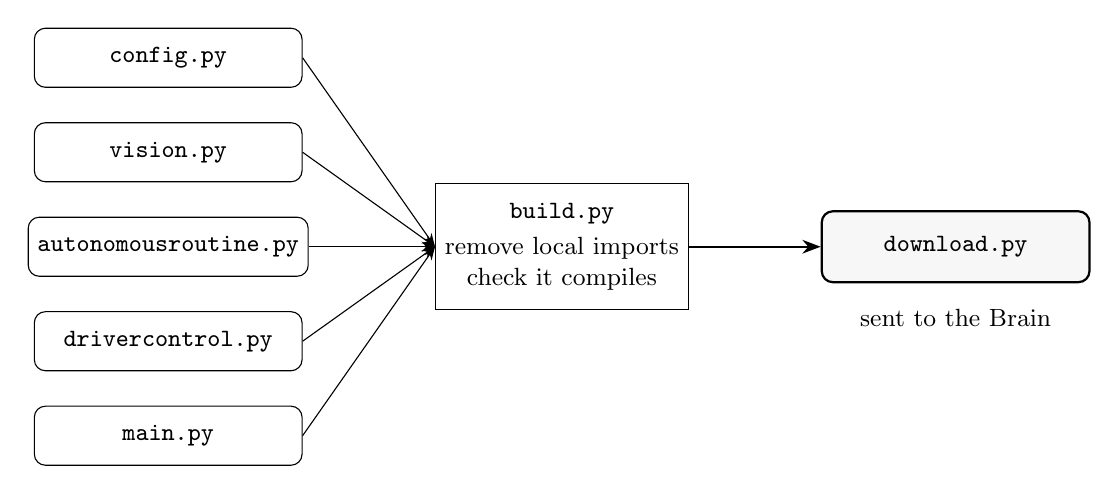
\begin{tikzpicture}[
      file/.style={draw, rounded corners, minimum width=3.4cm, minimum height=0.75cm, font=\ttfamily\small},
      outfile/.style={draw, thick, rounded corners, minimum width=3.4cm, minimum height=0.9cm, font=\ttfamily\small, fill=codebg},
      >={Stealth}]
    \node[file] (c) at (0,  2.4) {config.py};
    \node[file] (v) at (0,  1.2) {vision.py};
    \node[file] (a) at (0,  0.0) {autonomousroutine.py};
    \node[file] (d) at (0, -1.2) {drivercontrol.py};
    \node[file] (m) at (0, -2.4) {main.py};
    \node[draw, align=center, minimum width=3.2cm, minimum height=1.6cm, font=\small] (b) at (5,0)
      {\texttt{build.py}\\[2pt] remove local imports\\ check it compiles};
    \node[outfile] (o) at (10,0) {download.py};
    \node[font=\small, below=0.2cm of o] {sent to the Brain};
    \foreach \n in {c,v,a,d,m} \draw[->] (\n.east) -- (b.west);
    \draw[->, thick] (b) -- (o);
  \end{tikzpicture}
  \caption{\code{build.py} joins the five source files, in dependency order, into the single file the Brain runs (self-made).}
  \label{fig:build}
\end{figure}

The order matters. Python reads a file from top to bottom, so a function must be
defined before anything that uses it runs. Since every other file reads values
from \code{config.py}, it must come first. The order is stored in a list:

\lstinputlisting[firstline=12,firstnumber=12,lastline=19,caption={Module order and import patterns in \code{build.py}, lines 12--19.},label=lst:buildorder]{../build.py}

The two regular expressions (text patterns) match the import lines that would
break on the robot. \code{LOCAL_IMPORT} matches imports of our own files, which
are no longer needed once everything is in one file. \code{VEX_IMPORT} matches
\code{from vex import *}, which every file repeats; the build keeps just one
copy at the top. The main loop then removes those lines from each file and
joins what remains:

\lstinputlisting[firstline=36,firstnumber=36,lastline=59,caption={Flattening and checking in \code{build.py}, lines 36--59.},label=lst:buildloop]{../build.py}

Line 54 is a safety check. \code{compile()} asks Python to read the combined
file without running it. If the combination has a syntax error, the build stops
with a clear message instead of writing a broken file. Without this check, the
error would only appear on the robot, with a line number pointing into the
nearly 900-line generated file, which is much harder to trace back to the original
source.

Note: \code{download.py} is generated, so it must never be edited by hand. Any
edit would be overwritten the next time \code{build.py} runs. We still commit it
to git, so that a fresh copy of the project can be downloaded to a robot
immediately at a competition, even without Python installed.

\section{Selecting a Mode}
\label{sec:modes}

At a real competition, the field control system tells the robot when to run
autonomous and when to hand over to the driver. During practice there is no
field control, so \code{main()} chooses one mode by hand:

\lstinputlisting[firstline=13,firstnumber=13,lastline=23,caption={Mode selection in \code{src/main.py}, lines 13--23.},label=lst:main]{\src{main.py}}

Exactly one line is left uncommented. The diagnostic modes
(\code{scan_ports}, \code{vision_report}, \code{cone_detector}) and the
calibration mode (\code{turn_tuner}) are kept here so that any of them can be
run on the robot by changing one line, rather than by writing a separate
program.

\section{Summary}

\begin{enumerate}
  \item The robot has two green-cartridge drive motors, two red-cartridge
    manipulator motors and an AI Vision sensor (\sref{sec:hardware}).
  \item The code is split into five files, with every tunable number kept in
    \code{config.py} (\sref{sec:layout}).
  \item The Brain runs only one file, so \code{build.py} joins the five files
    and checks the result compiles before it is downloaded (\sref{sec:build}).
\end{enumerate}

We now explain how the robot moves during the autonomous period.

\chapter{Autonomous Movement}
\label{ch:movement}

During the autonomous period, nobody is steering. The robot can only follow a
list of instructions such as ``drive 1000~mm forward, then turn 90 degrees
right''. This chapter explains how the program turns those instructions into
motor rotations, how we calibrate the result, and how the final autonomous
routine uses them.

\section{Encoders and Wheel Degrees}
\label{sec:encoders}

Each V5 motor contains an \emph{encoder}, a sensor that counts how far the motor
shaft has turned, in degrees. The motor can be told ``turn exactly 1128
degrees'' and it will stop itself once the encoder reaches that number. The
robot has no sensor that measures distance along the floor directly, so every
autonomous movement must be converted into a number of shaft degrees first.

\section{The Original Approach}
\label{sec:original}

The program originally used the SDK's built-in \code{DriveTrain} class, which
does this conversion internally. It was constructed as follows (from commit
\commit{4f76b82}, since removed):

\begin{lstlisting}[caption={Original drivetrain construction, \code{src/main.py} at \commit{4f76b82}.},label=lst:olddt,numbers=none]
dt = DriveTrain(left_motor, right_motor, 300, 320, 320, MM)
\end{lstlisting}

The three numbers are the wheel travel, track width and wheelbase in
millimetres. However, these are the SDK's example values, not measurements of
our robot. Our wheels are 4-inch (101.6~mm) wheels, which travel about 319~mm
per revolution, not 300~mm. Since every movement depended on these numbers,
every autonomous distance and angle was wrong. We replaced \code{DriveTrain}'s
movement functions with our own maths (commit \commit{eb032a0}), so that every
step of the conversion is visible and can be checked.

\section{Driving Straight}
\label{sec:drive}

When a wheel turns once, the robot moves forward by the wheel's circumference,
$\pi D$, where $D$ is the wheel diameter. To move a distance $d$, the wheel must
therefore turn $d / (\pi D)$ revolutions, which is $360\,d/(\pi D)$ degrees.
Including the external gear ratio $G$ and a correction factor $S_d$, the number
of shaft degrees is
\begin{equation}
  \theta_{\text{drive}} = \frac{d}{\pi D} \times 360 \times G \times S_d .
  \label{eq:drive}
\end{equation}

$G$ is the number of motor revolutions per wheel revolution. Our wheels are
mounted directly on the motors, so $G = 1$. $S_d$ is \code{DRIVE_SCALE}, a
multiplier that absorbs small errors such as tyre squash or a slightly wrong
diameter. It starts at 1.00. Equation \eref{eq:drive} is implemented directly:

\lstinputlisting[firstline=9,firstnumber=9,lastline=11,caption={\code{wheel_degrees_for_distance()} in \code{src/autonomousroutine.py}, lines 9--11.},label=lst:drivedeg]{\src{autonomousroutine.py}}

\textbf{Worked example:} To drive $d = 1000$~mm with $D = 101.6$~mm,
\[
  \pi D = \pi \times 101.6 \approx 319.2~\text{mm},
  \qquad
  \theta_{\text{drive}} = \frac{1000}{319.2} \times 360 \approx 1128^\circ .
\]
So each wheel turns just over three full revolutions. The same function with
the SDK's default value of 300~mm would give $1200^\circ$, and the robot would
drive about 1064~mm instead of 1000~mm, an error of over 6\%.

\section{Turning in Place}
\label{sec:turn}

To turn on the spot, the two wheels spin in opposite directions. The robot then
rotates around the point halfway between its wheels, and each wheel travels
along a circle whose diameter is the \emph{track width} $W$, the distance between
the left and right wheels (\fref{fig:turn}).

\begin{figure}[h]
  \centering
  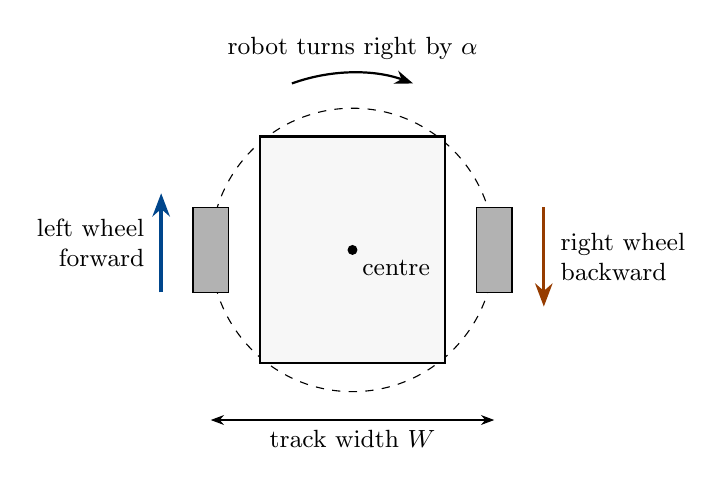
\begin{tikzpicture}[>={Stealth}, scale=0.9]
    \draw[dashed] (0,0) circle (2);
    \draw[thick, fill=codebg] (-1.3,-1.6) rectangle (1.3,1.6);
    \fill (0,0) circle (2pt) node[below right] {\small centre};
    \draw[fill=gray!60] (-2.25,-0.6) rectangle (-1.75,0.6);
    \draw[fill=gray!60] (1.75,-0.6) rectangle (2.25,0.6);
    \draw[<->] (-2,-2.4) -- node[below] {\small track width $W$} (2,-2.4);
    \draw[->, very thick, codekw] (-2.7,-0.6) -- (-2.7,0.8);
    \node[left, font=\small, align=right] at (-2.8,0.1) {left wheel\\forward};
    \draw[->, very thick, codest] (2.7,0.6) -- (2.7,-0.8);
    \node[right, font=\small, align=left] at (2.8,-0.1) {right wheel\\backward};
    \draw[->, thick] (110:2.5) arc (110:70:2.5);
    \node[font=\small] at (0,2.85) {robot turns right by $\alpha$};
  \end{tikzpicture}
  \caption{A right point turn, seen from above. Each wheel follows the dashed circle of diameter $W$ (self-made).}
  \label{fig:turn}
\end{figure}

One full spin moves each wheel along the whole circle, $\pi W$. A turn of
$\alpha$ degrees is the fraction $\alpha/360$ of a full spin, so each wheel
travels an arc of length
\begin{equation}
  s = \pi W \times \frac{\alpha}{360} .
  \label{eq:arc}
\end{equation}

Note: this is not doubled. It can look as if both wheels together must cover
$2\pi W$, but each wheel only covers its own half of the motion; the two sides
split the circle by moving in opposite directions. \code{AGENTS.md} warns
about this because it has been mistaken for an error before.

Converting the arc $s$ into shaft degrees in the same way as \eref{eq:drive},
with the turn correction factor $S_t$ (\code{TURN_SCALE}),
\begin{equation}
  \theta_{\text{turn}} = \frac{\pi W \alpha / 360}{\pi D} \times 360 \times G \times S_t
                       = \frac{W}{D}\,\alpha\, G\, S_t .
  \label{eq:turn}
\end{equation}

The $\pi$ and the 360 cancel, which leaves a neat result: the wheel turns
$W/D$ times as far as the robot does.

\lstinputlisting[firstline=13,firstnumber=13,lastline=16,caption={\code{wheel_degrees_for_turn()} in \code{src/autonomousroutine.py}, lines 13--16.},label=lst:turndeg]{\src{autonomousroutine.py}}

\textbf{Worked example:} For a 90° right turn, with $W = 320$~mm,
\[
  \theta_{\text{turn}} = \frac{320}{101.6} \times 90 \approx 3.15 \times 90 \approx 283^\circ .
\]
The left wheel turns $283^\circ$ forward and the right wheel $283^\circ$
backward. \code{turn()} does this by passing the same number to both sides with
opposite signs:

\lstinputlisting[firstline=39,firstnumber=39,lastline=47,caption={\code{drive()} and \code{turn()} in \code{src/autonomousroutine.py}, lines 39--47.},label=lst:driveturn]{\src{autonomousroutine.py}}

The right motor is declared \emph{reversed} in \code{config.py} (it faces the
other way on the robot), so ``forward'' means robot-forward on both sides. That
is why a negative number on the right side is what makes the robot turn.

\section{Stopping Accurately: HOLD versus BRAKE}
\label{sec:hold}

A V5 motor has three ways of stopping:

\begin{itemize}
  \item \textbf{COAST} cuts the power and lets the motor spin freely until
    friction stops it.
  \item \textbf{BRAKE} shorts the motor so it resists turning, which stops it
    quickly, but it stops resisting once it has stopped.
  \item \textbf{HOLD} actively pushes the motor back to its target position, even
    after it has arrived.
\end{itemize}

The original program used \code{BRAKE} during autonomous. The problem is that a
moving robot has momentum, so it slides slightly past its target. With
\code{BRAKE}, this overshoot is kept, and it adds up across every movement in the
routine. With \code{HOLD}, the motor notices that it has passed the target and
pulls back. \code{AGENTS.md} records that switching to \code{HOLD} removed most
of the original turn error. \code{move_wheels()} therefore sets \code{HOLD} before
every autonomous movement (lines 28--29 of \code{autonomousroutine.py}).

Driver control still uses \code{BRAKE}, because a driver expects the robot to
stop and stay where it stops, not pull back towards an old target.

\section{Timeouts}
\label{sec:timeouts}

Every movement has a \emph{timeout}, a maximum time after which the motor gives
up. This prevents the robot from pushing against an obstacle forever. The
original program used a flat 5-second timeout for every move. However, a long
drive can need more than 5 seconds, and the timeout then silently stops it
halfway with no error.

\textbf{Worked example:} A green-cartridge motor turns at up to 200~rpm, which is
$200 \times 360 / 60 = 1200$ degrees per second (\code{MOTOR_MAX_DPS}). At 50\%
speed, it turns 600 degrees per second. \code{drive(5000)} needs
$5000 / 319.2 \times 360 \approx 5639^\circ$, which takes about 9.4~s. In
5~s, the motor only reaches $5 \times 600 = 3000^\circ$, which is about 2660~mm,
or 53\% of the requested distance.

The timeout is now calculated from the movement itself:
\begin{equation}
  t_{\text{timeout}} = 2 \times \frac{\theta}{\omega} + 1~\text{s},
  \label{eq:timeout}
\end{equation}
where $\omega$ is the expected speed in degrees per second. The factor of 2
allows for the motor being slower than its theoretical speed, and the extra
second covers the time spent speeding up on short moves.

\lstinputlisting[firstline=18,firstnumber=18,lastline=21,caption={\code{move_timeout_ms()} in \code{src/autonomousroutine.py}, lines 18--21.},label=lst:timeout]{\src{autonomousroutine.py}}

For \code{drive(5000)} at 50\%, this gives $2 \times 9.4 + 1 = 19.8$~s, which is
long enough to complete the move but still stops a robot that is genuinely
stuck.

\section{Calibration}
\label{sec:calibration}

Equations \eref{eq:drive} and \eref{eq:turn} are only as accurate as the
measurements of $D$ and $W$. In practice, turns are also affected by
\emph{wheel scrub}: during a point turn the tyres slide sideways slightly, so the
encoders reach their target while the robot has turned less than intended.
Scrub cannot be predicted from the geometry, so instead of measuring it, we
absorb it into \code{TURN_SCALE}.

If we ask for a turn of $\alpha_{\text{asked}}$ and the robot actually turns
$\alpha_{\text{measured}}$, the corrected scale is
\begin{equation}
  S_{\text{new}} = S_{\text{old}} \times \frac{\alpha_{\text{asked}}}{\alpha_{\text{measured}}} .
  \label{eq:scale}
\end{equation}

\textbf{Worked example:} We ask for a full 360° spin with $S_t = 1.00$ and the
robot stops at 330°. Then $S_{\text{new}} = 1.00 \times 360/330 \approx 1.091$, so
every future turn is made about 9\% larger to compensate.

Measuring angles by eye is slow, so we wrote \code{turn_tuner()} (commit
\commit{eb032a0}) to do the calibration on the robot itself, using the
controller. Button A spins the robot one or more full turns and B spins it back.
The up and down arrows change \code{TURN_SCALE} by 0.010, and R1 and R2 change
it by 0.001 for fine adjustment. The driver keeps adjusting until the robot ends
a full spin facing exactly the way it started, then copies the value shown on
the screen into \code{config.py}. Button Y changes the test speed, because scrub
depends on speed; the scale should be tuned at the speed the routine actually
uses.

\section{Squaring to the Wall}
\label{sec:wallsquare}

Even with perfect calibration, an autonomous routine is only as good as its
starting position. If the robot starts angled by 3°, it will end up about
52~mm off course after driving 1~m. Human placement at the start of a match is
not precise enough to avoid this.

\code{square_to_wall()} solves this by using the field wall as a reference. The
robot reverses slowly into the wall. When one side touches first, that side
stops while the other keeps going, which rotates the robot until its back is
flat against the wall.

\lstinputlisting[firstline=168,firstnumber=168,lastline=184,caption={\code{square_to_wall()} in \code{src/autonomousroutine.py}, lines 168--184.},label=lst:wall]{\src{autonomousroutine.py}}

The robot knows it has reached the wall when both motors have \emph{stalled},
meaning their speed has dropped below 5\% even though they are still powered.
Three timings make this reliable:

\begin{itemize}
  \item \code{WALL_SQUARE_MIN_MS} (400~ms): stall checks are skipped at first,
    because a motor that has only just started is also moving slowly and would
    look stalled.
  \item \code{WALL_SQUARE_PUSH_MS} (300~ms): after both sides stall, the robot
    keeps pushing briefly, so that both sides are pressed flat rather than just
    touching.
  \item \code{WALL_SQUARE_MAX_MS} (2500~ms): if no wall is found, the robot
    gives up rather than reversing forever.
\end{itemize}

\section{The Autonomous Routine}
\label{sec:routine}

The final routine follows the path in \fref{fig:path}. The robot starts at S
with its back towards the wall, facing A.

\begin{figure}[h]
  \centering
  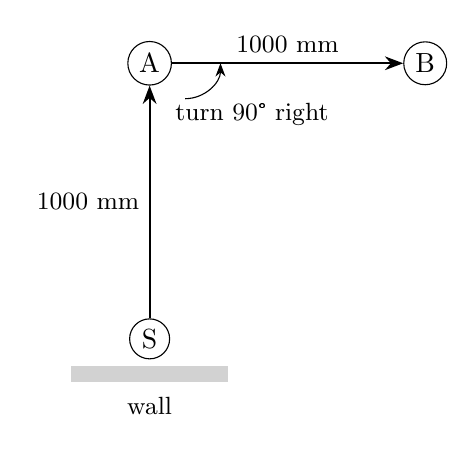
\begin{tikzpicture}[>={Stealth}, scale=1]
    \fill[gray!35] (-1.0,-0.55) rectangle (1.0,-0.35);
    \node[font=\small] at (0,-0.85) {wall};
    \node[circle, draw, fill=white, inner sep=2pt] (S) at (0,0) {S};
    \node[circle, draw, fill=white, inner sep=2pt] (A) at (0,3.5) {A};
    \node[circle, draw, fill=white, inner sep=2pt] (B) at (3.5,3.5) {B};
    \draw[->, thick] (S) -- node[left, font=\small] {1000 mm} (A);
    \draw[->, thick] (A) -- node[above, font=\small] {1000 mm} (B);
    \draw[->] (0.45,3.05) arc (-90:0:0.45);
    \node[font=\small] at (1.3,2.85) {turn 90° right};
  \end{tikzpicture}
  \caption{The S--A--B autonomous path (self-made).}
  \label{fig:path}
\end{figure}

\lstinputlisting[firstline=186,firstnumber=186,lastline=208,caption={Arm helpers and \code{autonomous()} in \code{src/autonomousroutine.py}, lines 186--208.},label=lst:auto]{\src{autonomousroutine.py}}

The steps are:

\begin{enumerate}
  \item Square to the wall, so the robot starts straight (\sref{sec:wallsquare}).
  \item Lift the arm 90 motor degrees and \code{HOLD} it, so it does not drag on
    the floor while driving.
  \item Drive 1000~mm to A, turn 90° right, and drive 1000~mm to B.
  \item Release the arm by switching it to \code{COAST}, so it drops under its
    own weight.
\end{enumerate}

A 300~ms \code{settle()} between moves lets the robot stop rocking, so that the
momentum of one move does not carry into the next.

\section{Summary}

\begin{enumerate}
  \item Distances and angles are converted into shaft degrees with
    \eref{eq:drive} and \eref{eq:turn}, using measured wheel and track sizes
    rather than the SDK's defaults.
  \item \code{HOLD} and proportional timeouts make each move end where it
    should (\sref{sec:hold}, \sref{sec:timeouts}).
  \item \code{TURN_SCALE} absorbs wheel scrub and is tuned on the robot with
    \code{turn_tuner()} (\sref{sec:calibration}).
  \item Squaring to the wall gives a repeatable starting position for the
    S--A--B routine (\sref{sec:wallsquare}, \sref{sec:routine}).
\end{enumerate}

We now explain the driver control half of the program.

\chapter{Driver Control}
\label{ch:driver}

In the driver control period, a person steers the robot with the controller.
The left stick drives, and the right stick moves the arm and claw. The program's
job is to turn stick positions into motor power in a way that feels smooth and
predictable. This chapter follows a stick reading through each processing step,
then explains the arm, the claw and the cone assist.

All of this happens inside \code{user_control()} in \code{src/drivercontrol.py},
which repeats every 20~ms (\code{LOOP_MS}), or 50 times per second.

\section{From Stick to Target Power}
\label{sec:stick}

A stick reports its position as a number from $-100$ to $100$. Three steps turn
this into a \emph{target} power for the drive.

\textbf{Deadband.} A stick rarely rests at exactly zero, so a released stick
might report 1 or $-1$. If this were passed to the motors, the robot would creep.
Readings smaller than \code{DEADBAND} (2) are therefore treated as zero.

\textbf{Squaring.} The reading is squared while keeping its sign:
\begin{equation}
  f = \frac{x\,|x|}{100} \times m ,
  \label{eq:square}
\end{equation}
where $x$ is the stick reading and $m$ is the speed multiplier. Squaring gives
the driver finer control near the centre, where precise movements happen, while
still reaching full power at the edge.

\textbf{Worked example:} With the stick halfway forward ($x = 50$) and the normal
multiplier $m = 0.5$, $f = 50 \times 50 / 100 \times 0.5 = 12.5\%$. Without
squaring, the same stick position would give 25\%. So the first half of the
stick's travel covers only the slowest quarter of the speed range, which makes
small adjustments much easier.

\textbf{Speed modes.} The multiplier $m$ depends on the right shoulder buttons:

\begin{table}[h]
  \centering
  \begin{tabular}{@{}lll@{}}
    \toprule
    Held & Multiplier & Use \\
    \midrule
    nothing & 0.50 (\code{SPEED_NORMAL}) & general driving \\
    R1      & 1.00 (\code{SPEED_BOOST})  & crossing the field quickly \\
    R2      & 0.25 (\code{SPEED_CRAWL})  & lining up precisely \\
    \bottomrule
  \end{tabular}
  \caption{Speed modes.}
  \label{tab:speeds}
\end{table}

The turning stick is processed in the same way, except that it is divided by 200
rather than 100, and multiplied by \code{TURN_NORMAL} (0.8) unless R1 is held.
This keeps turns gentler than forward movement in normal driving.

\section{Slew Limiting}
\label{sec:slew}

If the driver pushes the stick from zero to full in an instant, sending full
power straight to the motors would jolt the robot. This can make it tip, spin
its wheels, or throw a game object out of the claw. \emph{Slew limiting} stops
this by letting the power change by only a small step each loop.

\lstinputlisting[firstline=10,firstnumber=10,lastline=22,caption={\code{slew()} in \code{src/drivercontrol.py}, lines 10--22.},label=lst:slew]{\src{drivercontrol.py}}

There are two step sizes. Speeding up uses the smaller \emph{acceleration}
step, so the robot gets moving smoothly. Slowing down (or reversing) uses the
larger \emph{deceleration} step, so the robot still stops quickly when the
driver lets go. Line 12 decides which one applies: if the target has the
opposite sign to the current power, or is smaller in size, the robot is slowing
down.

\textbf{Worked example:} \code{FWD_ACCEL_STEP} is 4, so going from 0 to 100\% takes
$100 / 4 = 25$ loops, or $25 \times 20~\text{ms} = 500$~ms.
\code{FWD_DECEL_STEP} is 12, so stopping from 100\% takes about 9 loops, or
170~ms. Turning uses larger steps (8 and 20), because a slow-to-respond turn
feels sluggish to the driver.

\section{Balancing Forward and Turn}
\label{sec:taper}

In arcade drive, the left motor gets \textit{forward + turn} and the right motor
gets \textit{forward $-$ turn}. Two problems come from this.

\textbf{Turning too sharply at speed.} The same turn stick input that is useful
for spinning on the spot makes the robot swerve violently at full speed.
\code{turn_taper()} reduces the turn as the forward speed increases:
\begin{equation}
  g(f) = g_{\text{rest}} + (g_{\text{full}} - g_{\text{rest}}) \frac{|f|}{100} ,
  \label{eq:taper}
\end{equation}
with $g_{\text{rest}} = 1.00$ and $g_{\text{full}} = 0.35$. At rest the driver
gets the full turn; at full speed only 35\% of it; and at 50\% forward power,
$g = 1 + (0.35 - 1)(0.5) = 0.675$.

\textbf{Clipping.} A motor cannot exceed 100\%. If forward is 80 and turn is 40,
the left motor would be asked for 120 and is cut to 100, while the right motor
gets 40. The robot's average forward speed drops from 80 to 70, so the driver
loses speed just by turning. \code{fit_turn()} prevents this by shrinking the turn
instead of the forward power:

\lstinputlisting[firstline=37,firstnumber=37,lastline=44,caption={\code{fit_turn()} in \code{src/drivercontrol.py}, lines 37--44.},label=lst:fitturn]{\src{drivercontrol.py}}

\textbf{Worked example:} With forward 80 and turn 40, there is $100 - 80 = 20$
of room left. With \code{FORWARD_PRIORITY} at 0.8, the allowed turn is
$40 + (20 - 40)(0.8) = 24$. The motors receive $80 + 24 = 104$ (cut to 100) and
$80 - 24 = 56$, an average of 78 instead of 70. Most of the forward speed is
kept, and the robot still turns.

Holding R1 skips both the taper and \code{fit_turn()}, giving the driver raw,
unrestricted control when they want it.

\section{Arm and Claw}
\label{sec:manipulator}

The right stick's vertical axis moves the arm and its horizontal axis moves the
claw. The arm is squared and slew-limited in the same way as the drive, because
a heavy arm that starts or stops suddenly swings and can shake loose what it is
carrying. The claw is not slew-limited, since it is light and needs to respond
immediately.

Both use \code{HOLD} when stopped (\code{manipulator_init()} in
\code{config.py}), so the arm does not sag under its own weight. The claw's
torque is limited with \code{CLAW_TORQUE}, and the claw only gets 60\% power
(\code{CLAW_SPEED}), because once the claw has closed on an object, extra power
only stalls the motor and makes it overheat. For tuning, \code{CLAW_DIAGNOSTIC}
prints the claw motor's current and temperature to the Brain screen five times
per second. This is wrapped in a \code{try} block (lines 53--58), so that if the
SDK cannot report these values, the diagnostic fails quietly instead of
stopping the drive in the middle of a match.

There are optional software limits on the arm (\code{ARM_USE_LIMITS}). When
enabled, the arm refuses to move further past its lowest or highest position,
but is always allowed to move back.

\section{Cone Assist}
\label{sec:assist}

The cone assist lets the driver press one button to make the robot find the cone
and turn to face it. The left and right arrows start a search to the left or
right. It uses the AI Vision sensor, which is explained in \cref{ch:vision};
here we only describe how the assist behaves.

The assist moves through three states:

\begin{enumerate}
  \item \textbf{Searching:} spin slowly (15\%) in the chosen direction. The speed
    is kept low because the camera's image blurs when the robot spins quickly,
    and a blurred cone is not recognised.
  \item \textbf{Aligning:} once the cone has been seen in 3 frames in a row,
    turn towards it with a power proportional to how far off-centre it is.
  \item \textbf{Centred:} once the cone has been within 4 pixels of the centre for
    3 frames in a row, stop and rumble the controller twice.
\end{enumerate}

If the cone disappears for 5 frames in a row while aligning, the assist goes
back to searching.

\lstinputlisting[firstline=77,firstnumber=77,lastline=82,caption={\code{assist_steer()} in \code{src/drivercontrol.py}, lines 77--82.},label=lst:steer]{\src{drivercontrol.py}}

The turn power is \code{ASSIST_STEER_KP} (0.12) multiplied by the error in
pixels. This is called \emph{proportional control}~\cite{astrom2008}: a big error
gives a fast turn, and a small error gives a slow turn, so the robot slows down
as it approaches the target and does not overshoot. However, a very small power
is not enough to overcome friction, and the robot would stop just short of the
centre. The power is therefore never allowed below 4\% (\code{ASSIST_MIN_TURN}),
and it is capped at 15\% so the image does not blur.

\textbf{Worked example:} If the cone is 100 pixels right of centre, the power is
$0.12 \times 100 = 12\%$. At 10 pixels, $0.12 \times 10 = 1.2\%$, which is raised to
the minimum of 4\%.

\subsection{Cancelling}

The driver must always be able to take back control instantly, because a stuck
assist during a match could cost the game. Every loop, the assist checks all
twelve buttons and both sticks; any button, or any stick pushed past 20, cancels
it straight away.

This created a problem. The button that \emph{starts} the assist is still being
held down on the assist's first loop, so it would immediately cancel the assist.
The \code{released} flag fixes this: the start button is ignored until it has
been let go once. The reverse problem happens in \code{user_control()}: a
button held down after cancelling would immediately start the assist again. The
start is therefore \emph{edge-triggered}, meaning it only fires at the moment the
button goes from not-pressed to pressed:

\lstinputlisting[firstline=174,firstnumber=174,lastline=188,caption={Edge-triggered start in \code{user_control()}, \code{src/drivercontrol.py}, lines 174--188.},label=lst:edge]{\src{drivercontrol.py}}

The assist also uses \code{spin()}, which sets a speed and returns immediately,
rather than \code{spin_for()}, which waits until a movement finishes. A function
that waits cannot check the buttons in the meantime, so it could not be
cancelled.

\section{Summary}

\begin{enumerate}
  \item Stick readings are deadbanded, squared and scaled by a speed mode
    (\sref{sec:stick}).
  \item Slew limiting ramps power up gently but lets it drop quickly
    (\sref{sec:slew}).
  \item The turn is tapered at speed and shrunk before it can clip, keeping
    forward speed (\sref{sec:taper}).
  \item The cone assist searches, aligns with proportional control, and can be
    cancelled by any input (\sref{sec:assist}).
\end{enumerate}

We now explain how the robot recognises the cone.

\chapter{AI Vision}
\label{ch:vision}

The AI Vision sensor is a camera with its own processor. It does not send whole
images to the Brain. Instead, it finds areas of the image that match colours we
have described, and reports a list of \emph{objects}: where each one is and how
big it is. This chapter explains how we describe the cone to the sensor, how
the program picks the cone out of the sensor's reports, and the diagnostic tools
we built when the sensor did not work.

\section{How the Sensor Reports Objects}
\label{sec:sensor}

The sensor's image is 320 pixels wide and 240 pixels tall. For each object it
finds, it reports:

\begin{itemize}
  \item \code{id}: which colour (or colour code) matched;
  \item \code{centerX}, \code{centerY}: the centre of the object, in pixels;
  \item \code{width}, \code{height}: the size of the object's bounding box, the
    smallest rectangle that contains it.
\end{itemize}

These numbers are enough for our purposes. \code{centerX} tells us whether the
cone is to the left (below 160) or right (above 160) of the robot, and
\code{width} tells us roughly how close it is, since a closer cone looks wider.

\section{Describing the Cone}
\label{sec:describe}

Our cone is half yellow and half blue. We give the sensor two \emph{colour
descriptions}, one for each half, and one \emph{colour code}, which matches only
when the two colours are found next to each other. The colour code is more
reliable than either colour alone, because many things on a field are yellow or
blue, but very few are yellow directly beside blue.

\lstinputlisting[firstline=151,firstnumber=151,lastline=160,caption={Colour descriptions in \code{src/config.py}, lines 151--160.},label=lst:colours]{\src{config.py}}

Each \code{Colordesc} gives an id, a red--green--blue (RGB) value, and two
tolerances: how far the hue (the shade of colour) and the saturation (how vivid
it is) may differ from that value and still count as a match. The RGB values
were sampled from the AI Vision Utility, a VEX tool that shows the camera's view
on a laptop. The tolerances are wide (hue 40, saturation 1.00), which helps the
sensor recognise the cone in different lighting, but might also match objects
that are not the cone.

These descriptions are passed to \code{AiVision()}, which sends them to the sensor
when the program starts. Line 160 then switches colour detection on. Both of
these details were discovered the hard way, as described in
\sref{sec:ch-silent}.

\section{Finding the Cone}
\label{sec:findcone}

\code{find_cone()} is the one function that every other part of the program uses
to look for the cone. It returns the cone's object, or \code{None} if there is no
cone in view.

\lstinputlisting[firstline=9,firstnumber=9,lastline=26,caption={\code{find_cone()} in \code{src/vision.py}, lines 9--26.},label=lst:findcone]{\src{vision.py}}

It first asks the sensor for every colour code it can see (line 14). It ignores
any that are not the cone code, and any smaller than 6 by 6 pixels, since a tiny
match is more likely to be noise than a cone. If several cones remain, it
returns the largest, because the largest is most likely the nearest.

The minimum size of 6 pixels was originally 20. We lowered it because a cone on
the far side of the field is only about 15 pixels wide, so the robot could not
see distant cones at all (commit \commit{6c3a1b7}).

\section{The Colour-Pair Fallback}
\label{sec:colourpair}

At a distance or in poor lighting, the sensor sometimes recognises both colours
but fails to recognise the code that combines them. When this happens,
\code{find_cone()} falls back to \code{find_color_pair()}, which does the
combination itself:

\lstinputlisting[firstline=36,firstnumber=36,lastline=56,caption={\code{find_color_pair()} in \code{src/vision.py}, lines 36--56.},label=lst:pair]{\src{vision.py}}

It finds the largest yellow object and the largest blue object. It then checks
that they are close together: their centres must be no further apart than the
largest side of either object (lines 49--51). If they are, it builds one box that
surrounds both (lines 52--56).

This merged box matters. An earlier version returned only the yellow half, so
the robot aimed at the middle of the yellow half instead of the middle of the
cone, and judged distance using half the cone's real width. Merging the two
halves into one box fixed both problems (commits \commit{8471b29} and
\commit{f1f4d77}).

The box is returned as a \code{ConeBox} (lines 28--34), a small class with the
same field names as a real sensor object. This means code that uses
\code{find_cone()} does not need to know which method found the cone.

\section{Confirming a Sighting}
\label{sec:confirm}

A single frame can contain a false match, for example a flash of light that
briefly looks yellow. Acting on every single sighting would make the robot
twitch. The program therefore waits for the cone to appear in
\code{VISION_CONFIRM_FRAMES} (3) frames in a row before believing it is there. At
one frame every 50~ms, this adds only 150~ms of delay. \code{cone_detector()}
(lines 58--98 of \code{vision.py}) uses the same idea in reverse: the cone must be
missing for 3 frames before the robot reports it as lost.

\section{Diagnostic Tools}
\label{sec:diagnostics}

When the sensor did not detect anything, there were several possible causes: a
wrong port, an unplugged cable, the colours not being loaded, or the program not
running at all. We built two tools to tell these apart without a laptop.

\subsection{Vision Report}

\code{vision_report()} draws the sensor's status on the Brain screen four times
per second:

\begin{itemize}
  \item a \textbf{tick counter} that goes up each time it redraws, which proves
    the program is running;
  \item \code{installed()}, which is \code{True} if a sensor is plugged into the
    configured port;
  \item the sensor's \textbf{timestamp}, which changes with every new frame, which
    proves the sensor is sending data;
  \item the number of \textbf{codes} and \textbf{colours} found, and the details of
    each object.
\end{itemize}

Each line rules out one cause. For example, if the tick climbs and the timestamp
changes but the counts stay at zero with the cone in view, then the program,
cable and sensor all work, and the problem must be the colour settings. This is
exactly what the screen showed on 22 September (\sref{sec:ch-silent}).

\subsection{Port Scanner}
\label{sec:portscan}

\code{scan_ports()} finds which port the sensor is on, which is useful because
the port in \code{config.py} was originally a guess:

\lstinputlisting[firstline=150,firstnumber=150,lastline=160,caption={Port probing in \code{scan_ports()}, \code{src/vision.py}, lines 150--160.},label=lst:scan]{\src{vision.py}}

It tries to create a sensor on each of the 21 ports. A port counts as a sensor
only if it reports \code{installed()} \emph{and} its timestamp changes over
100~ms; a port with nothing on it will not produce new frames. The
\code{try}/\code{except} block skips any port that causes an error, so one bad
port does not stop the scan.

\section{Summary}

\begin{enumerate}
  \item The sensor reports each matching object's position and size
    (\sref{sec:sensor}).
  \item The cone is described as a yellow--blue colour code, declared in code and
    sent to the sensor at start-up (\sref{sec:describe}).
  \item \code{find_cone()} returns the largest cone, falling back to merging a
    nearby yellow and blue object (\sref{sec:findcone}, \sref{sec:colourpair}).
  \item On-screen diagnostics and a port scanner find faults without a laptop
    (\sref{sec:diagnostics}).
\end{enumerate}

Having described the final program, we now describe how it developed over
time.

\chapter{Timeline}
\label{ch:timeline}

This chapter gives an overview of when each part of the program was built. The
dates and times come from the git history; all times are local (UTC+2).

\section{Overview}

\begin{figure}[h]
  \centering
  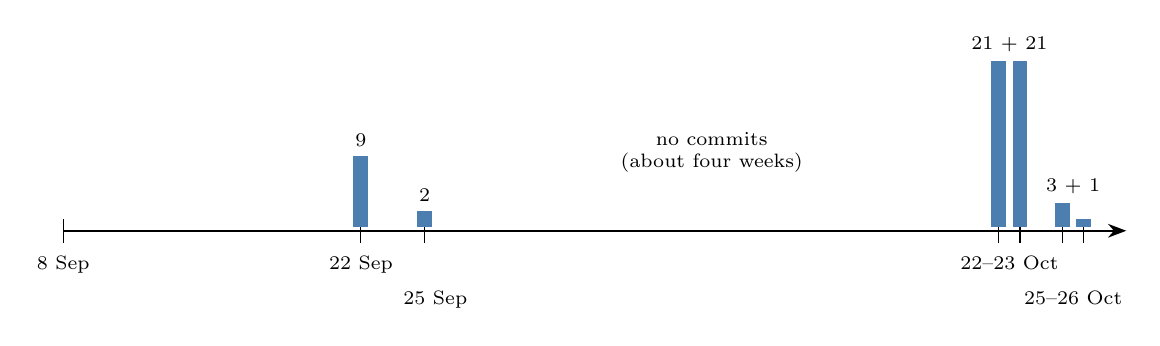
\begin{tikzpicture}[x=0.27cm, >={Stealth}]
    % Day 0 = 8 Sep, day 48 = 26 Oct.
    \draw[->, thick] (0,0) -- (50,0);
    % Bar height is 0.1 per commit.
    \draw (0,-0.15) -- (0,0.15);
    \foreach \d/\n in {14/9, 17/2, 44/21, 45/21, 47/3, 48/1} {
      \draw (\d,-0.15) -- (\d,0.15);
      \fill[codekw!70] (\d-0.35,0.05) rectangle (\d+0.35,0.05+0.1*\n);
    }
    \node[below, font=\scriptsize] at (0,-0.2) {8 Sep};
    \node[below, font=\scriptsize] at (14,-0.2) {22 Sep};
    \node[below, font=\scriptsize] at (17.5,-0.65) {25 Sep};
    \node[below, font=\scriptsize] at (44.5,-0.2) {22--23 Oct};
    \node[below, font=\scriptsize] at (47.5,-0.65) {25--26 Oct};
    \node[above, font=\scriptsize] at (14,0.95) {9};
    \node[above, font=\scriptsize] at (17,0.25) {2};
    \node[above, font=\scriptsize] at (44.5,2.15) {21 + 21};
    \node[above, font=\scriptsize] at (47.5,0.35) {3 + 1};
    \node[font=\scriptsize, align=center] at (30.5,1.0) {no commits\\(about four weeks)};
  \end{tikzpicture}
  \caption{Commits per day. Bar height shows the number of commits (self-made).}
  \label{fig:timeline}
\end{figure}

\begin{table}[h]
  \centering
  \begin{tabularx}{\textwidth}{@{}llcX@{}}
    \toprule
    Date & Day & Commits & Focus \\
    \midrule
    8 Sep 2026  & Mon & --  & Project created in VEXcode \\
    22 Sep 2026 & Mon & 9   & Accurate movement, file split and build step, first vision work \\
    25 Sep 2026 & Thu & 2   & Getting the vision sensor to detect the cone \\
    22 Oct 2026 & Thu & 21  & Autonomous that searches for the cone and drives to it \\
    23 Oct 2026 & Fri & 21  & Making the cone approach reliable \\
    25 Oct 2026 & Sun & 3   & Fixed S--A--B autonomous; cone search moved to driver control \\
    26 Oct 2026 & Mon & 1   & Repository published \\
    \bottomrule
  \end{tabularx}
  \caption{Summary of development days.}
  \label{tab:days}
\end{table}

The work happened in short, intense sessions rather than evenly over time. This
matches how a robotics team works in practice: most changes need the robot on a
practice field, so programming happens when the team meets.

\section{8 September: Project Created}

The VEXcode project was created on 8 September at 19:09 (recorded as
\code{creationDate} in the project settings). It was not yet under git, so the
next two weeks are not recorded commit by commit. By 21 September, a working
single-file program existed with arcade drive, slew limiting, the arm and claw,
and a basic autonomous routine. An older 177-line version was also kept as
\code{main.py.bak}.

\section{22 September: Foundations}

The first four commits all have a time of 15:21, which shows they were saved
together in one batch at the start of the session, rather than one at a time
while the work was being done.

\begin{itemize}
  \item \commit{4f76b82}: the existing program was saved unchanged, as a restore
    point in case any later change made things worse.
  \item \commit{eb032a0}: autonomous movement was rewritten with explicit maths,
    \code{HOLD}, proportional timeouts and the turn tuner (\cref{ch:movement}).
  \item \commit{78005ed}: first AI Vision cone detection.
  \item \commit{0607385}: the program was split into five files, with
    \code{build.py} to rejoin them (\cref{ch:structure}).
  \item \commit{165d475}, \commit{7043f53}: the README and AGENTS documents were
    written, and long comments were moved out of the code into them.
  \item \commit{2e1cf54}: the turn tuner's screen flicker was fixed.
  \item \commit{b4624fd}, \commit{91a2514}: the vision diagnostic was moved to
    the Brain screen, which revealed that colour detection was switched off.
\end{itemize}

\section{25 September: Making Vision Work}

\begin{itemize}
  \item \commit{08c26bb}: the colours were declared in code, after we found they
    had never reached the sensor.
  \item \commit{a2bfc94}: the port scanner was added.
\end{itemize}

\section{22 October: Searching for the Cone}

After about four weeks without commits, the goal changed: the autonomous routine
should find the cone and drive up to it by itself. This session used an AI coding
assistant, GitHub Copilot, from 16:46 to 17:28, then Claude from 17:32. Commits
were made every one to three minutes, which reflects a fast loop: change a
number, build, download, test on the robot, repeat.

The work moved through three phases: searching (spinning in a circle until the
cone is seen), approaching (driving towards it), and finally stopping to measure
before each turn.

\section{23 October: Making the Approach Reliable}

The second session (15:48 to 17:44) followed the same loop, with Claude. Almost
every commit fixes a failure seen in the previous test run: spinning past the
cone, not seeing the cone from far away, wobbling left and right when close,
losing the cone partway, and false readings. By the end of the day, the routine
was much more robust, but still not fully reliable.

\section{25 October: Change of Strategy}

\begin{itemize}
  \item \commit{76b036f}: the program was moved to download slot 3.
  \item \commit{cf781d1}: the cone-hunting autonomous was replaced with the fixed
    S--A--B path and wall squaring (\sref{sec:routine}). The cone alignment was
    moved into driver control as the cone assist (\sref{sec:assist}). This
    removed 622 lines and added 350.
  \item \commit{cc730b7}: the documentation was updated to match.
\end{itemize}

\section{26 October: Published}

\commit{448d4f1} added a heading to the README and marks the point at which the
repository was pushed online.

We now look at the main challenges in detail.


\bibliographystyle{unsrt}
\bibliography{references}

\end{document}
